\subsection{Datenstruktur}
Die Datenstruktur der Anwendung besteht grundsätzlich aus drei abstrakten und fünf konkreten Klassen. Die abstrakten Klassen sind Entitäten, organisationsbasierende Entitäten und verlinkbare Entitäten. Die absoluten Klassen sind Nutzer, Organisation, Level, Gruppe und Aufgabe.

\vspace{20pt}
\begin{center}
    \begin{minipage}{1\linewidth}
        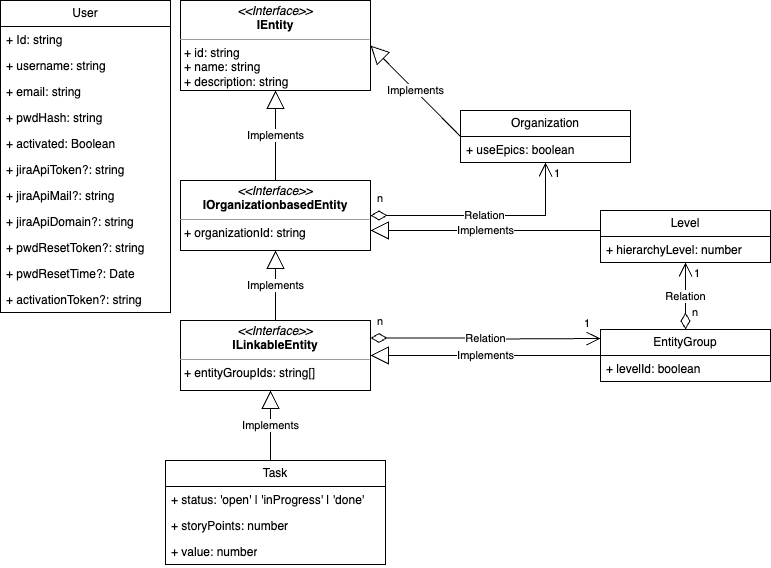
\includegraphics[width=\linewidth]{classDiagramm}
        \captionof{figure}{UML-Diagramm der Datenstruktur}
    \end{minipage}
\end{center}
\vspace{20pt}

Jede absolute Klasse, außer die Nutzer, erben von einer oder mehreren abstrakten Klassen. Entitäten sind allgemeine Objekte innerhalb der Anwendung und stellen die Grundlage der in der Datenbank gespeicherten Datenobjekte dar. Alle Klassen außer Nutzer sind solche Entitäten und implementieren das Interface \verb|IEntity|, welches eine ID zur eindeutigen Identifikation und einen Namen für die Darstellung für den Nutzer beinhaltet. Organisationen und Levels sind direkte Erben dieser Klasse. Die nächste Abstraktionsstufe sind die organisationsbasierenden Entitäten. Diese implementieren zu dem \verb|IEntity| Interface noch \verb|IOrganizationBasedEntity|, welches die ID einer Organisation voraussetzt und die Entität direkt von einer Organisation abhängig macht. Die letzte Abstraktionsstufe sind die verlinkbaren Entitäten. Diese implementieren zu dem \verb|IOrganizationBasedEntity| Interface noch \verb|ILinkableEntity|, welches eine Liste von IDs voraussetzt, mit dem gespeichert wird, mit welchen anderen verlinkbaren Entitäten das Objekt verlinkt ist. Aufgaben und Gruppen sind solche verlinkbare Entitäten.

\subsection{Backend-Architektur}
Das Backend ist eine REST-API, geschrieben mit Node.js und Express in TypeScript und verwendet mongoose als Datenbank-API für MongoDB. Die Architektur beschreibt den Datenfluss mit drei allgemeinen Komponenten: Router, Controller und Service.
Der Router bestimmt für einen Request welche Funktion eines Controllers aufgerufen wird. Die aufgerufene Controller-Funktion beinhaltet die Business-Logik, die an den Request gebunden ist und führt diese aus. Um Daten aus der Datenbank zu holen oder die geholten Daten zu modifizieren gibt es für jede Datenklasse einen Service, der die benötigten Datenbankoperationen implementiert und somit von der Business-Logik trennt. Für die Interaktion mit der Datenbank muss außerdem ein sogenanntes Model definiert werden, welches die Beschreibung der Klasse also der Type in TypeScript mit der Datenbank-Collection und den Objekten darin verknüpft.

\vspace{20pt}
\begin{center}
    \begin{minipage}{1\linewidth}
        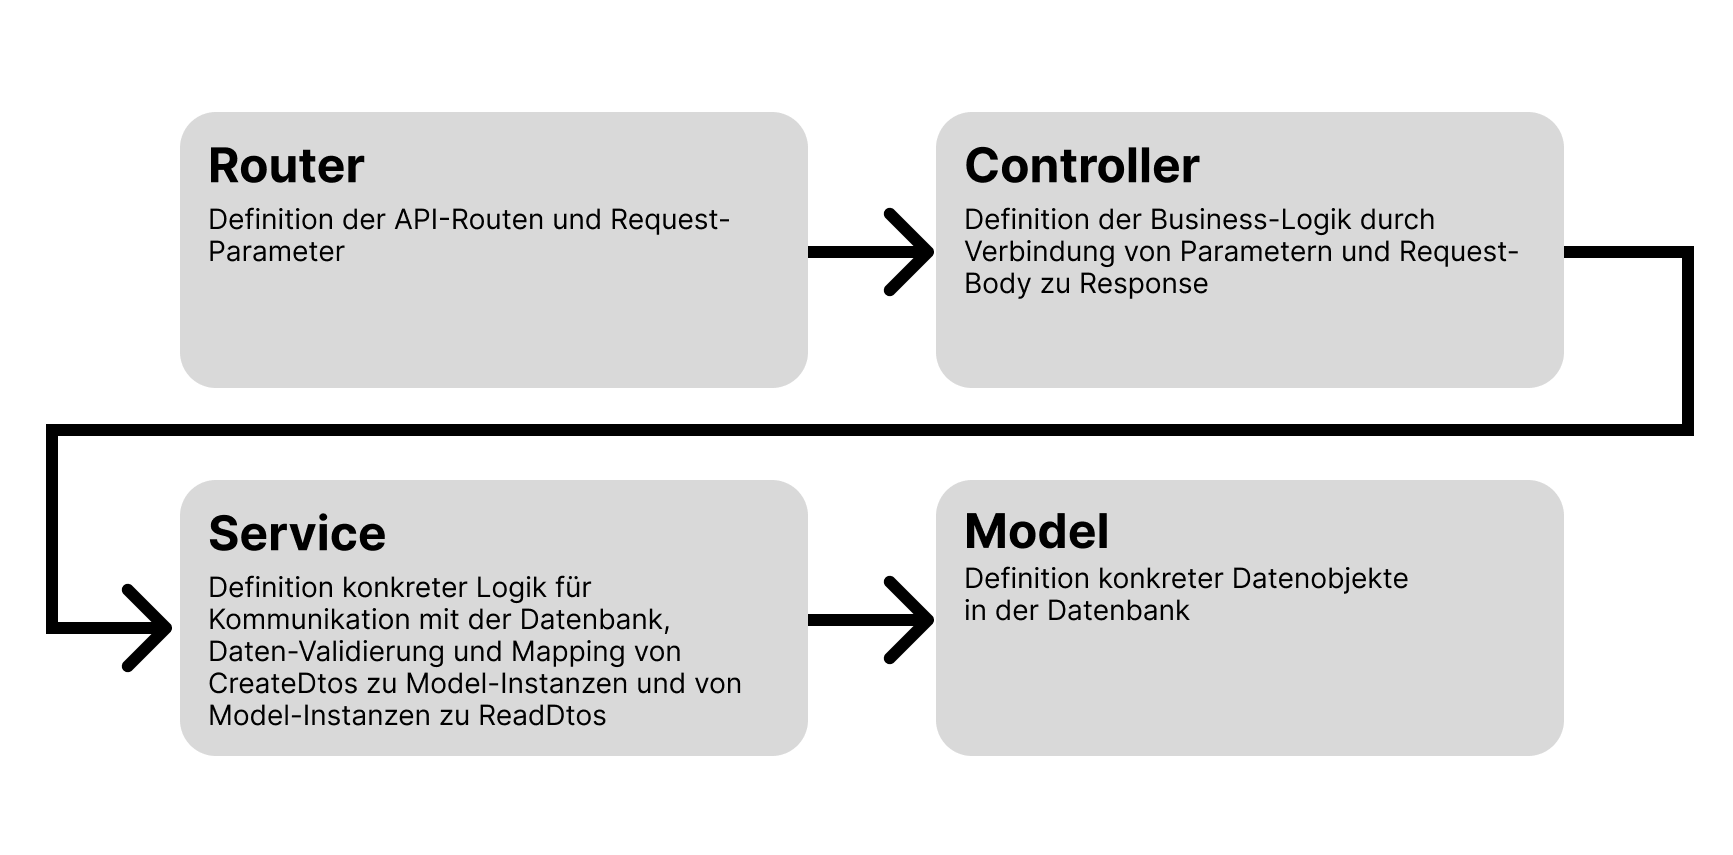
\includegraphics[width=\linewidth]{BE-Struktur}
        \captionof{figure}{Backend Architektur}
    \end{minipage}
\end{center}
\vspace{20pt}

Für die konkrete Kommunikation mit der REST-API werden zu den konkreten Datenobjekten innerhalb der Datenbank zwei weitere Klassen je Objekt-Klasse definiert. Diese Klassen sind sogenannte Data transfer Objects (DTO). DTOs dienen dazu die Kommunikation zu generalisieren und definieren die Daten, die der Konsument der API durch einen Request erhalten kann und die Daten, die ein Konsument der API zur Verfügung stellen kann, um z. B. ein neues Objekt in der Datenbank zu erstellen. Die zusätzlichen Klassendefinitionen werden durch diese zwei Anwendungsfälle in Read- und Create-/Update-DTOs unterteilt. Wie Create-/Update-DTOs zu einem internen Model gemappt werden und wie aus einem internen Model ein Read-Dto gemappt wird, definiert ebenfalls der zum Model zugehörige Service.

Der Aufbau des Backends gleicht dem Aufbau der Klassen-Abstraktion. Es gibt für jede abstrakte Klasse eine Struktur welche jeweils eine abstrakte Implementierung für Router, Controller, Services und Model beinhalten.
Zudem gibt es fünf absolute Strukturen für jede der fünf absoluten Klassen, welche von den verschiedenen abstrakten Strukturen erben.


\vspace{20pt}
\begin{center}
    \begin{minipage}{1\linewidth}
        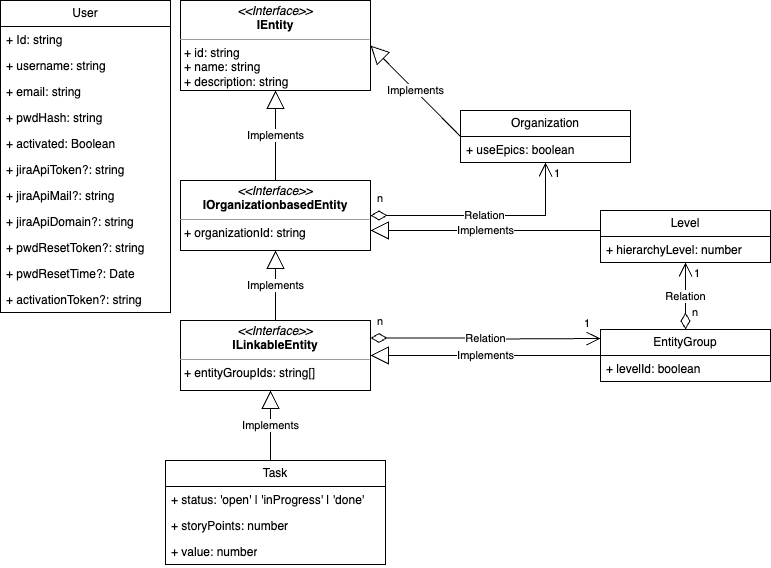
\includegraphics[width=\linewidth]{classDiagramm}
        \captionof{figure}{Abbildung der BE-Struktur}
    \end{minipage}
\end{center}
\vspace{20pt}

hier noch eine detaillierte Beschreibung der Strukturen ????

Eine vollständige Dokumentation der API im Swagger-Format ist unter \url{https://116.203.140.167.nip.io/api-docs/} verfügbar. Dort sind die für den Client zugänglichen Routen inklusive der benötigten Parameter und den zurückgegebenen Daten dokumentiert.

\subsection{Benutzeroberfläche}
Zur initialen Planung wurde zunächst der UX-Entwurf verwendet um die grobe Struktur der Benutzeroberfläche zu entwickeln. Durch die spezifische Entwicklung verschiedener Features sind immer wieder Lücken im Entwurf aufgefallen und wurden duch weitere UI-Elemente erweitert um Funktionalitäten abzudecken, die zuvor nicht innerhalb des Prototypen bedacht wurden. Bis zum fertigen Prototypen haben sich viele der konkreten UI-Elemente verändert, allerdings blieb die Seitenstruktur also welche Informationen auf welches Seite dargestellt wurden identisch.

Für die Implementierung wurde als Frontend-/UI-Framework Vue.js verwendet. Vue.js ist eine Framwork für die Entwicklung von Single-Page-Webanwendungen. Es ist ein JavaScript-Framework, welches auf dem Model-View-ViewModel (MVVM) basiert. Die UI wurde also in verschiedene Komponenten zerteilt. Die Komponenten werden in zwei Kategorien unterteilt: Views und Components. Views sind logisch voneinander getrennte Seiten der Anwendung, während Components kleinere Bestandteile der Views zur vereinfachung der in der View benötigten Logik oder wiederverwendbare UI-Elemente sind. Zur weiteren Strukturierung werden hier noch sogenannte Layouts verwendet. Layouts stellen die Grundstruktur der Anwendung dar, welche von mehreren Views verwendet wird.

Die Anwendung teilt sich zunächst in zwei solcher Layouts: Authentifizierung und eigentliche Anwendung.

Das Layout der Authentifizierung beschreibt nur die Positionierung der relevanten Elemente in der Mitte des Bildschirms, da sich alle Seiten der Authentifizierung diese Eigenschaft teilen.
Das Layout der eigentlichen Seite teilt die Seite in drei Teile, den Header, den Inhalt und einen Footer. Der Header beinhaltet die Navigationsleiste, die den Nutzer durch die Anwendung führt und oben rechts ein Aktionsmenü mit dem der Nutzer sich jederzeit ausloggen kann oder in die Einstellungen bzw. sein Profil navigieren kann. Der Inhalt ist der Bereich in dem die verschiedenen Views dargestellt werden. Der Footer beinhaltet Informationen über den aktuell eingeloggten Nutzer und seine Verbindung zu Jira.

\subsection{Visualisierung/Datendarstellung}
Für die generelle Visualisierung der gesamten Daten einer Organisation dient das Dashboard, welches den komplexesten Teil der Anwendung darstellt.

Hier werden alle Gruppen der Organisation Hierarchisch sortiert dargestellt und ihre Verknüpfungen untereinander visualisiert.
Um die Übersicht bei vielen Gruppen beizubehalten werden die Gruppen innerhalb einer hierarchischen Ebene nach ihren Verbindungen zu den darüberliegenden Gruppen sortiert, sodass Gruppen die mit der gleichen Gruppe in der Ebene darüber verknüpft sind nebeneinander dargestellt werden und die Verbindungslinien somit möglichst kurz und übersichtlich dargestellt.

\vspace{20pt}
\begin{center}
    \begin{minipage}{1\linewidth}
        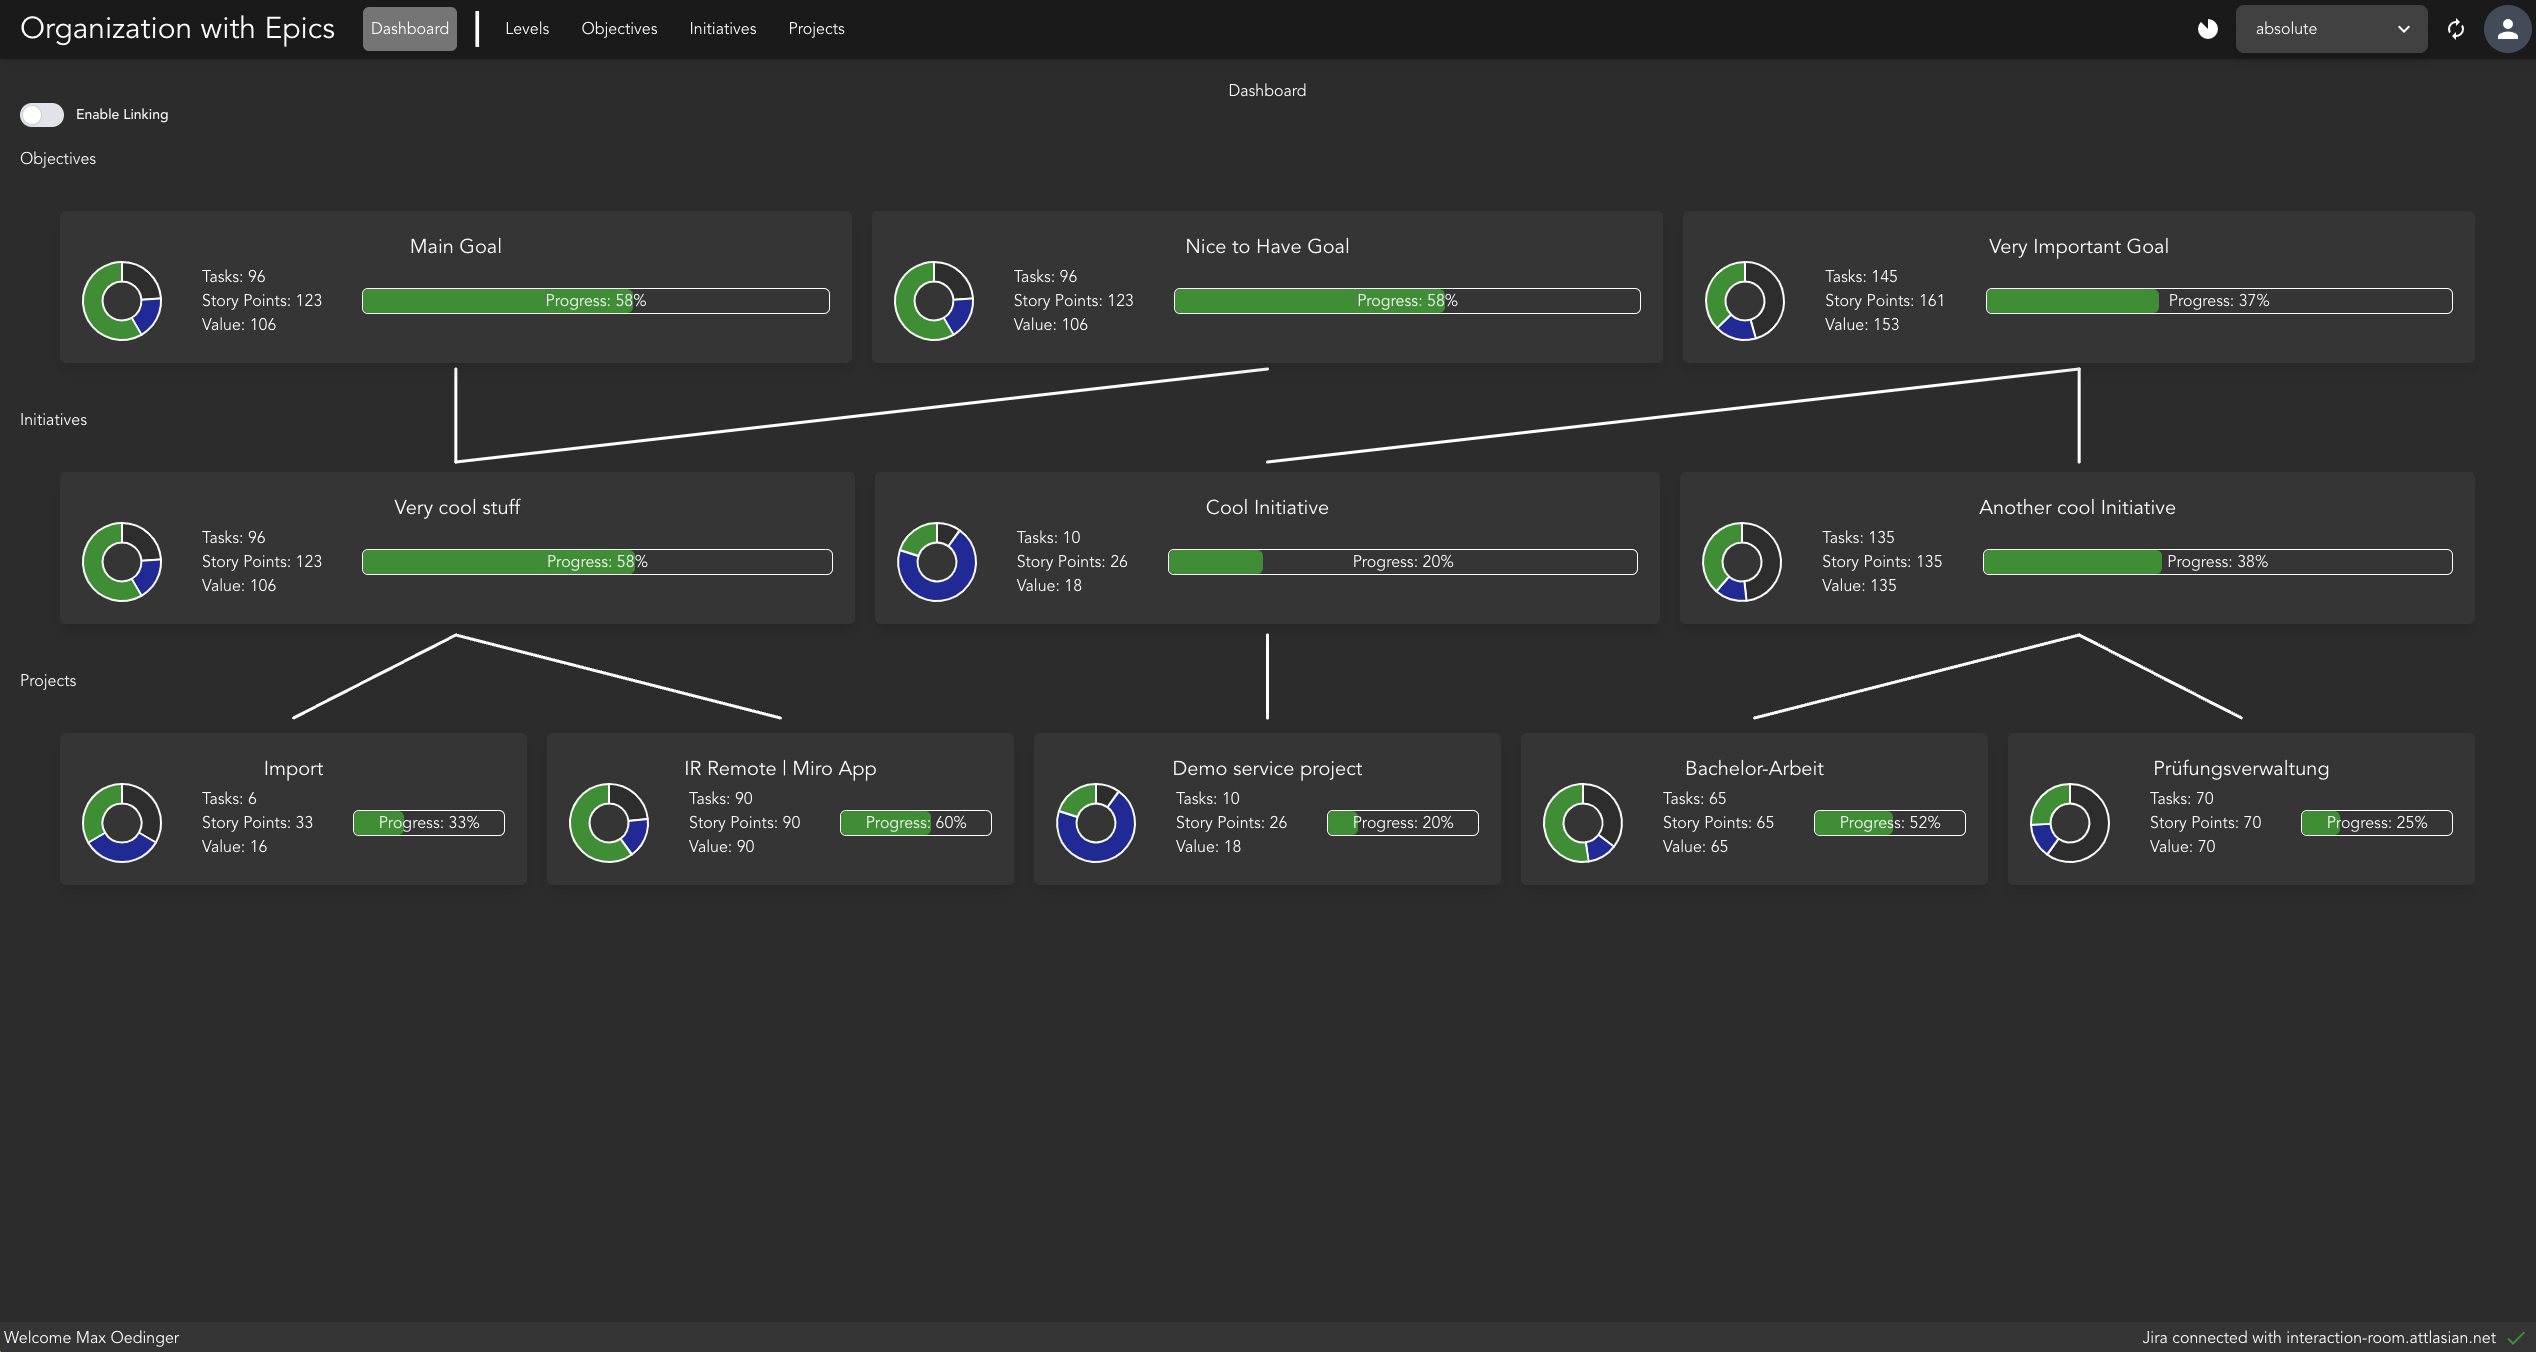
\includegraphics[width=\linewidth]{Dashboard_full}
        \captionof{figure}{Dashboard}
    \end{minipage}
\end{center}
\vspace{20pt}

Um die Verbindungslinien darzustellen wurde ein svg-Element im Hintergrund der Seite verwendet, welches die Verbindungslinien unabhängig von anderen Elementen auf der Seite darstellen kann. Die Start- und Endkoordinaten der Linien werden durch Positionen der Gruppen innerhalb der Seite berechnet. Dabei muss zusätzlich beachtet werden, wenn ein Level so viele Gruppen beinhaltet, dass sich einige Gruppen außerhalb des sichtbaren Bereichs befinden und durch einen Scroll in den sichtbaren bereich bewegt werden können. In diesem Fall müssen die Koordinaten der Linien entsprechend der Scroll-Position der verschobenen Gruppen neu berechnet werden.

\vspace{20pt}
\begin{center}
    \begin{minipage}{1\linewidth}
        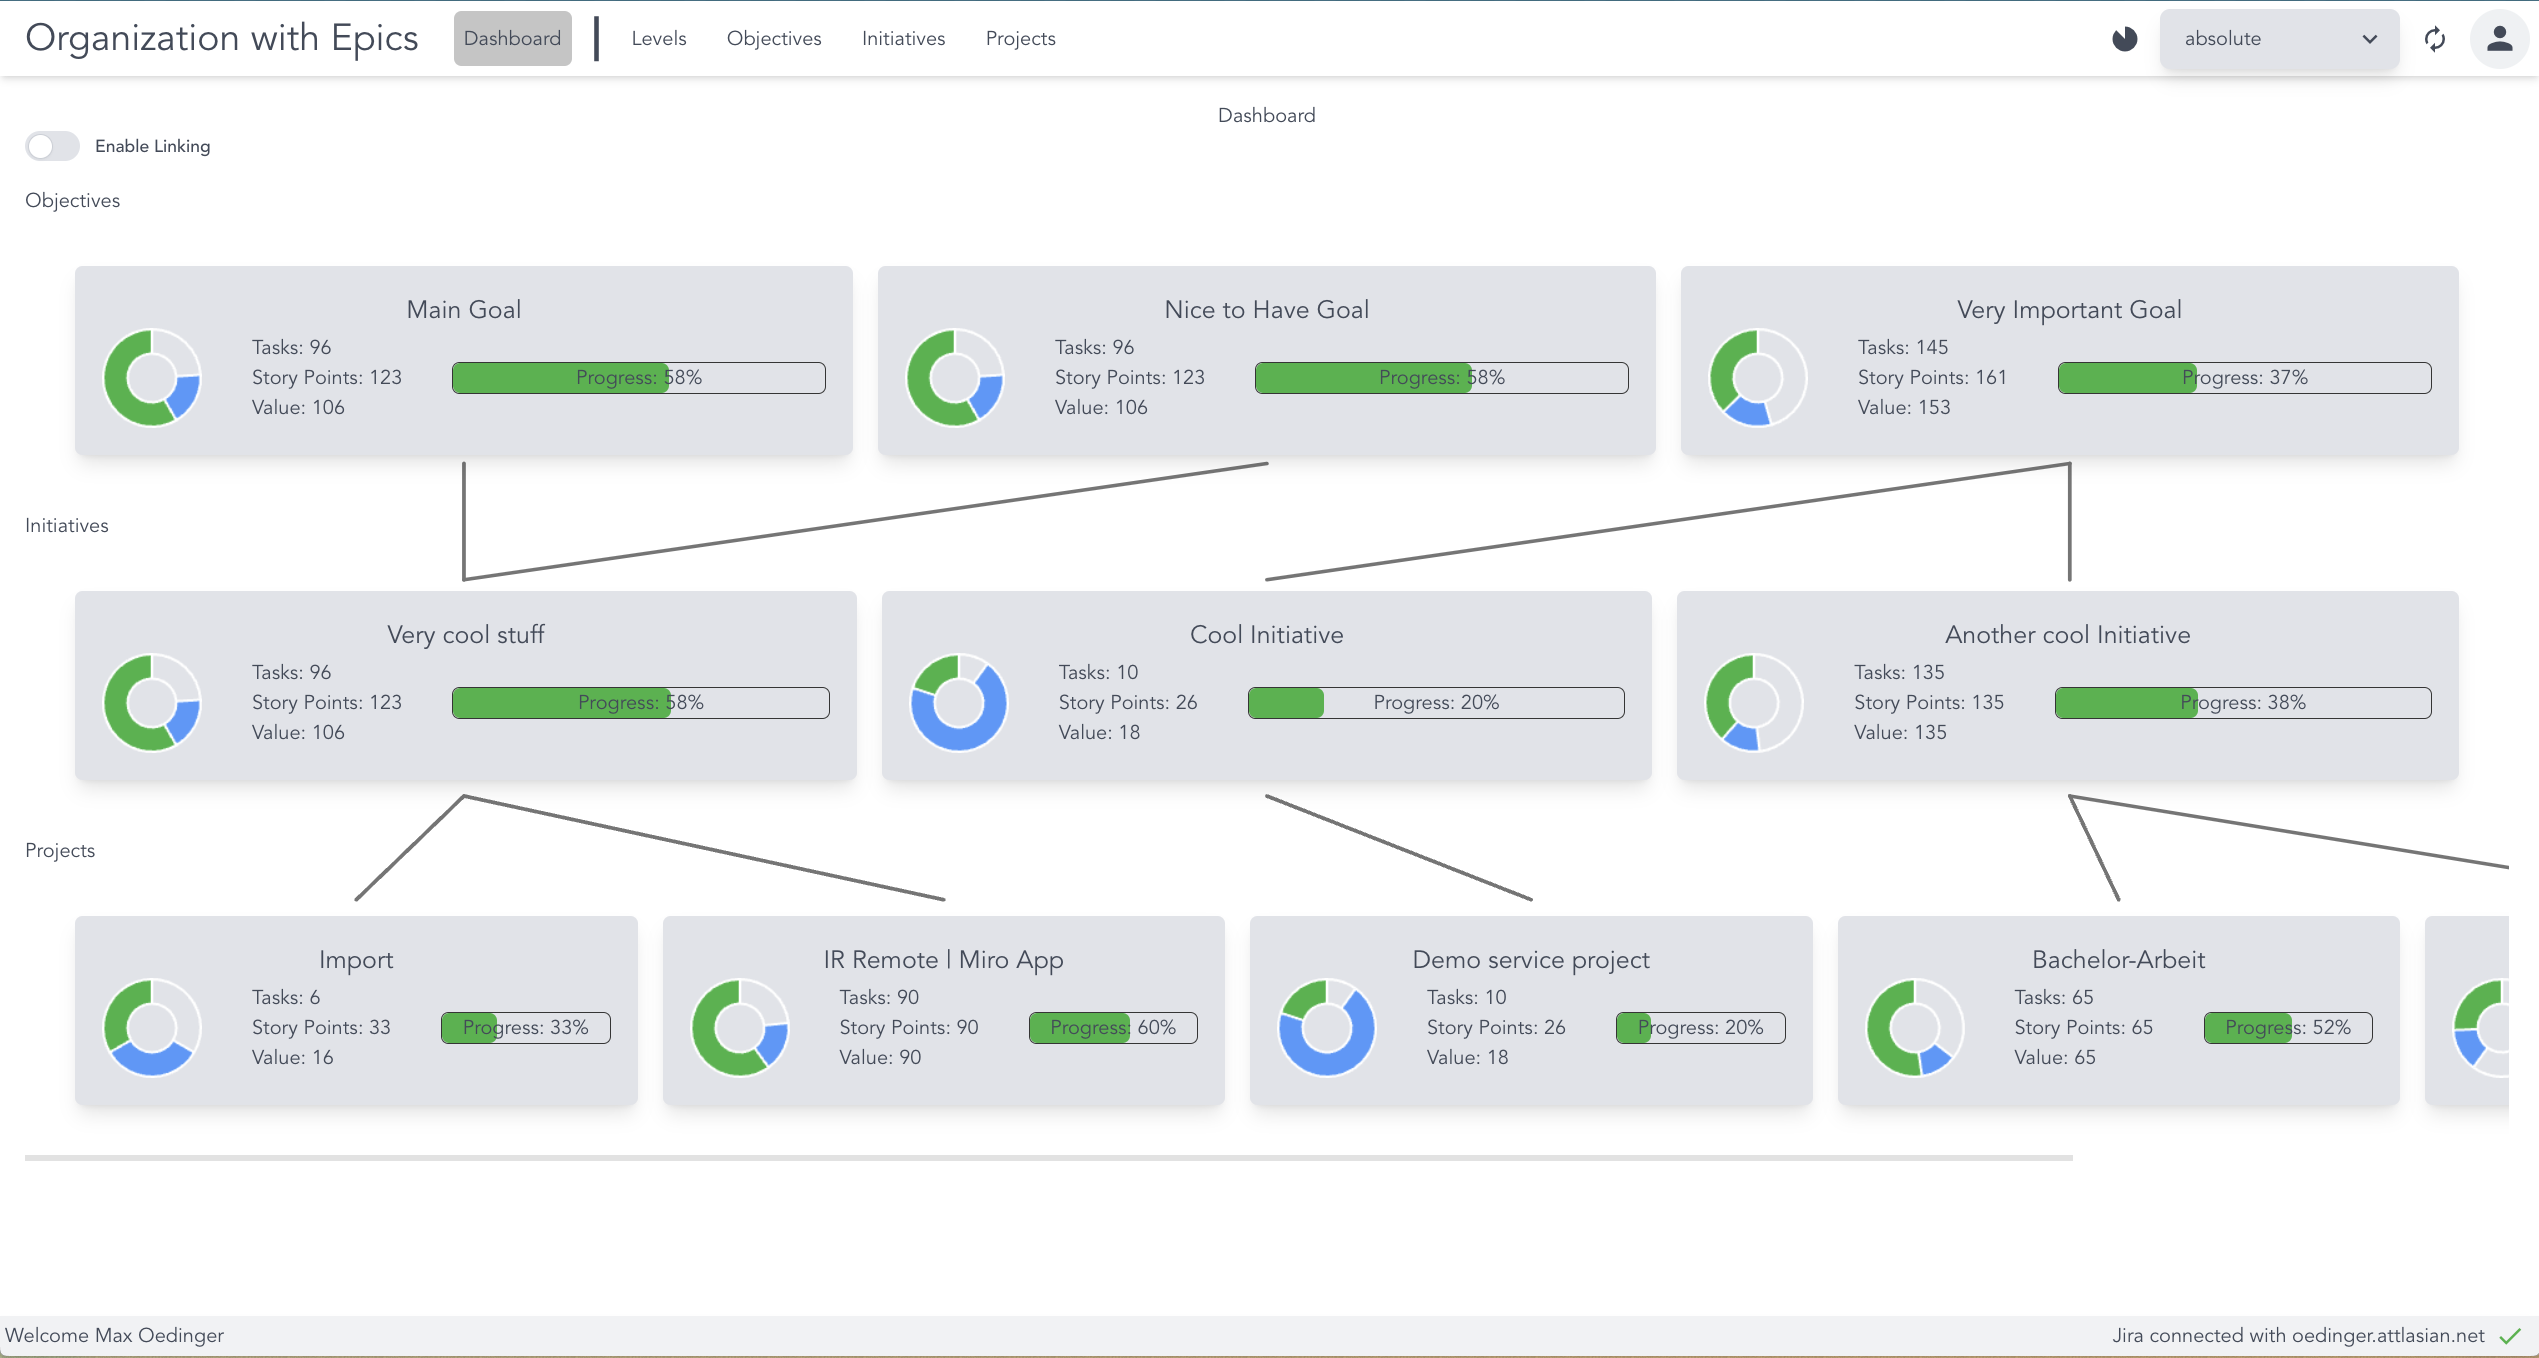
\includegraphics[width=\linewidth]{Dashboard_withScroll}
        \captionof{figure}{Dashboard mit scrollbaren Gruppen}
    \end{minipage}
\end{center}
\vspace{20pt}

Der Nutzer hat die Möglichkeit Verlinkung über ein Toggle zu aktivieren, wodurch über jeder Gruppe die verlinkt werden kann ein Punkt erscheint, den der Nutzer mit Drag and Drop verwenden kann um die Gruppe mit einer anderen Gruppe zu verbinden.
Anhand der Start-Position und aktuellen Position des Mauszeigers wird währenddessen eine neue Linies dargestellt, die dem Nutzer zeigt wie die Verbindung aussieht die er erzeugt. Anschließend werden die Verbindungsli
nien anhand der neuen Positionen der Gruppen erneut berechnet.

Zusätzlich zu den Linien kann der Nutzer den Mauszeiger über eine Gruppe bewegen, wodurch die Gruppe und die Gruppen die mit dieser Gruppe verknüpft sind, inklusieve aller relevanten Verbindungslinien blau hervorgehoben werden.

\vspace{20pt}
\begin{center}
    \begin{minipage}{1\linewidth}
        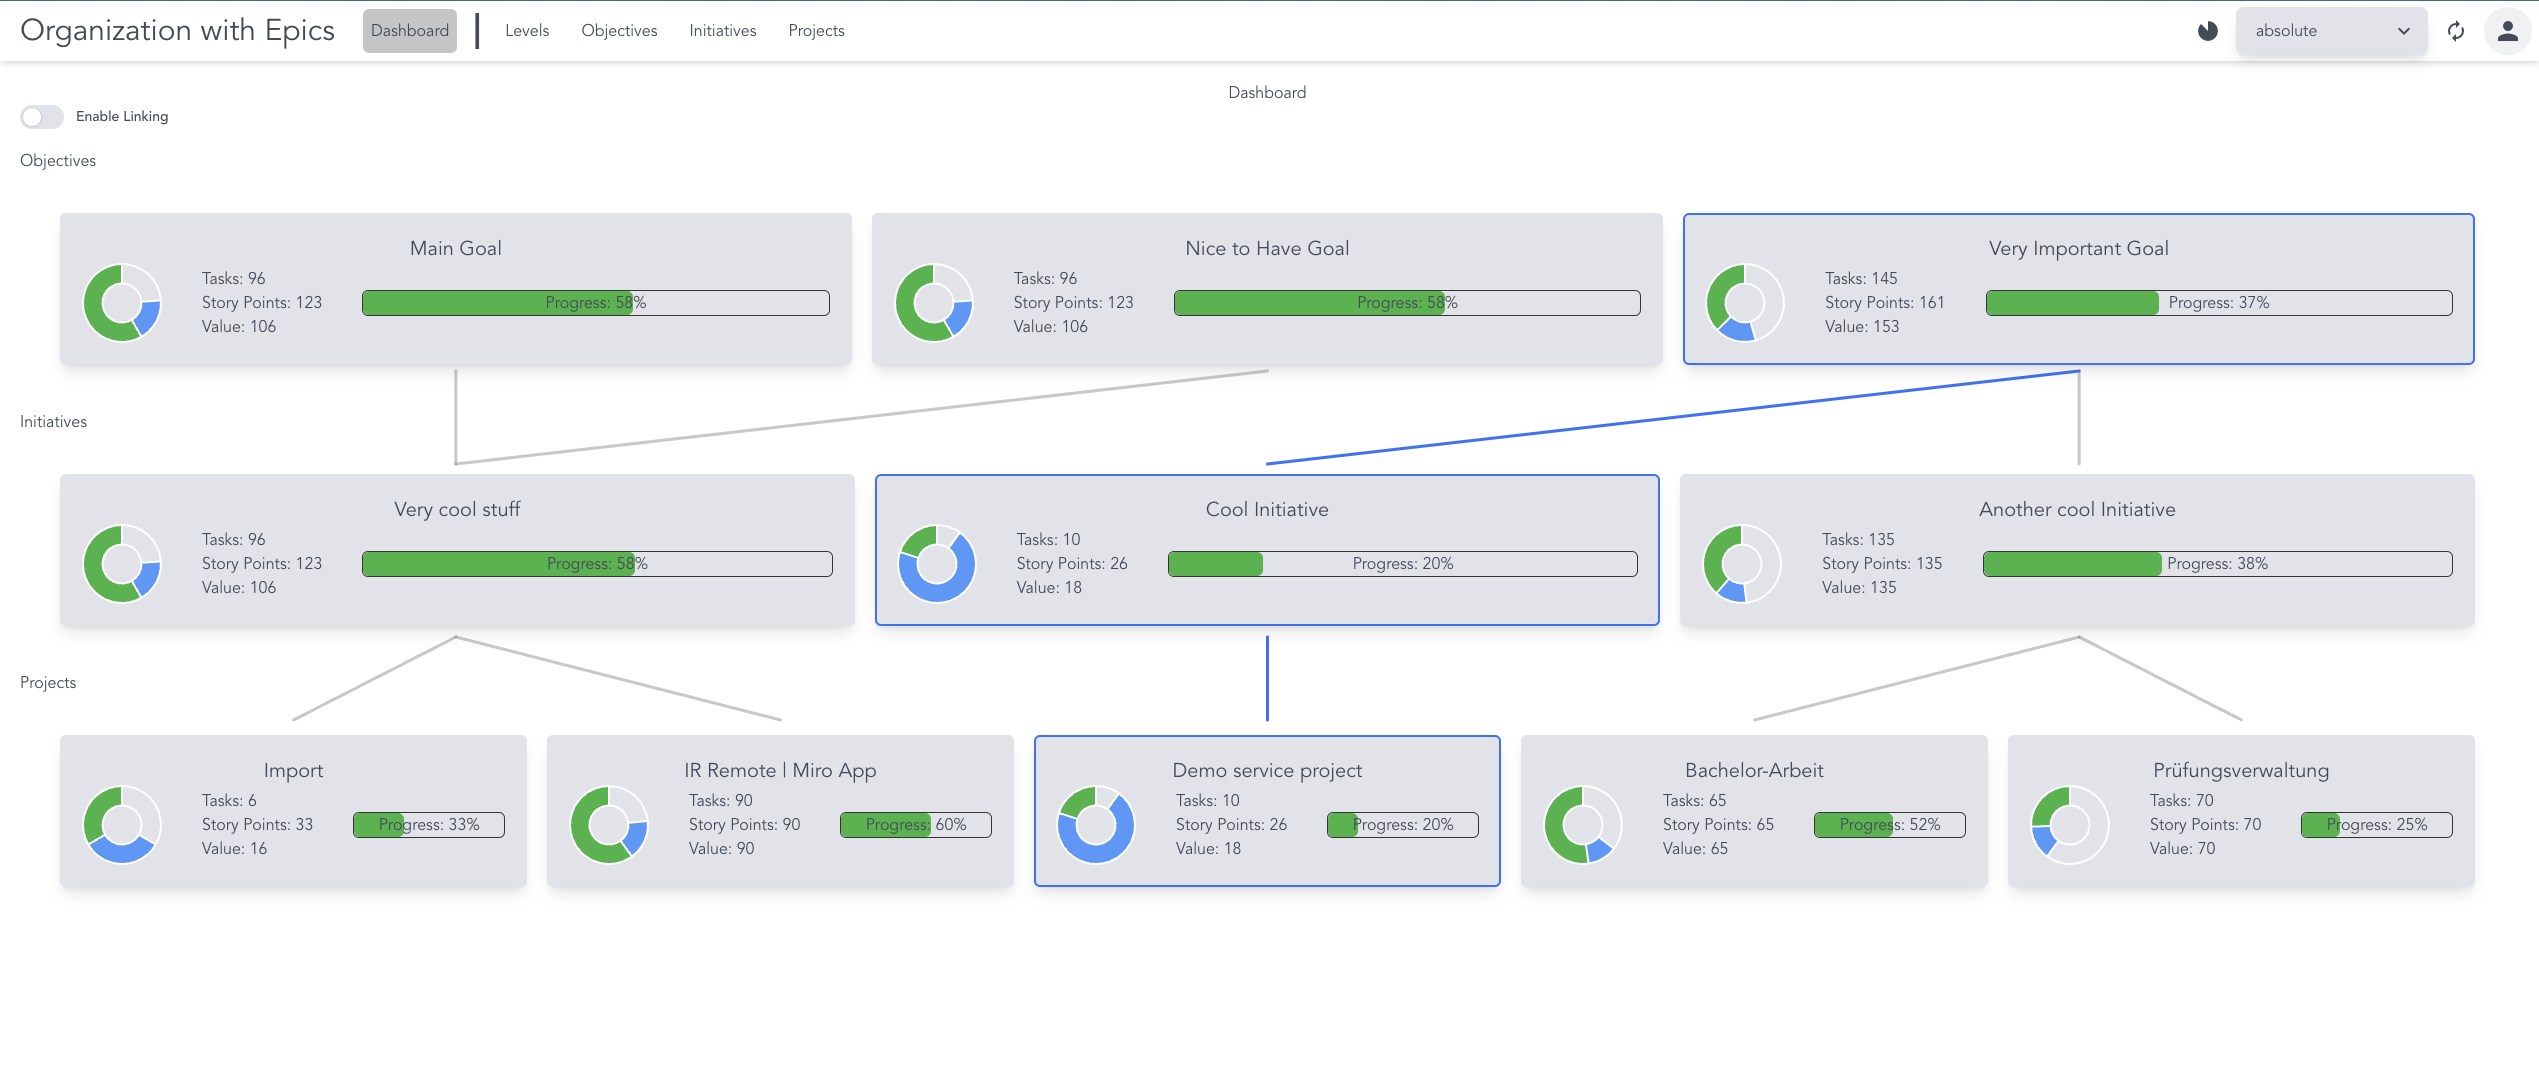
\includegraphics[width=\linewidth]{Dashboard_withHighlighting}
        \captionof{figure}{Dashboard mit hervorgehobenen Gruppen}
    \end{minipage}
\end{center}
\vspace{20pt}

\subsection{CI/CD}
Für eine schnelle und einfache Möglichkeit die Anwendung als produktive Anwendung zu testen und verbesserungen zu deployen wurde eine CI/CD-Pipeline mit GitHub-Actions eingerichtet. Die GitHub-Action definiert, wann die Pipeline ausgeführt werden soll und welche Schritte in der Pipeline ausgeführt werden sollen. Der Trigger für die Pipeline ist hier das Mergen und daraus resultierenden Schließen eines Pullrequests der als Ziel den main-Branch des Repositories hat.

\vspace{20pt}
\begin{center}
    \begin{minipage}{1\linewidth}
        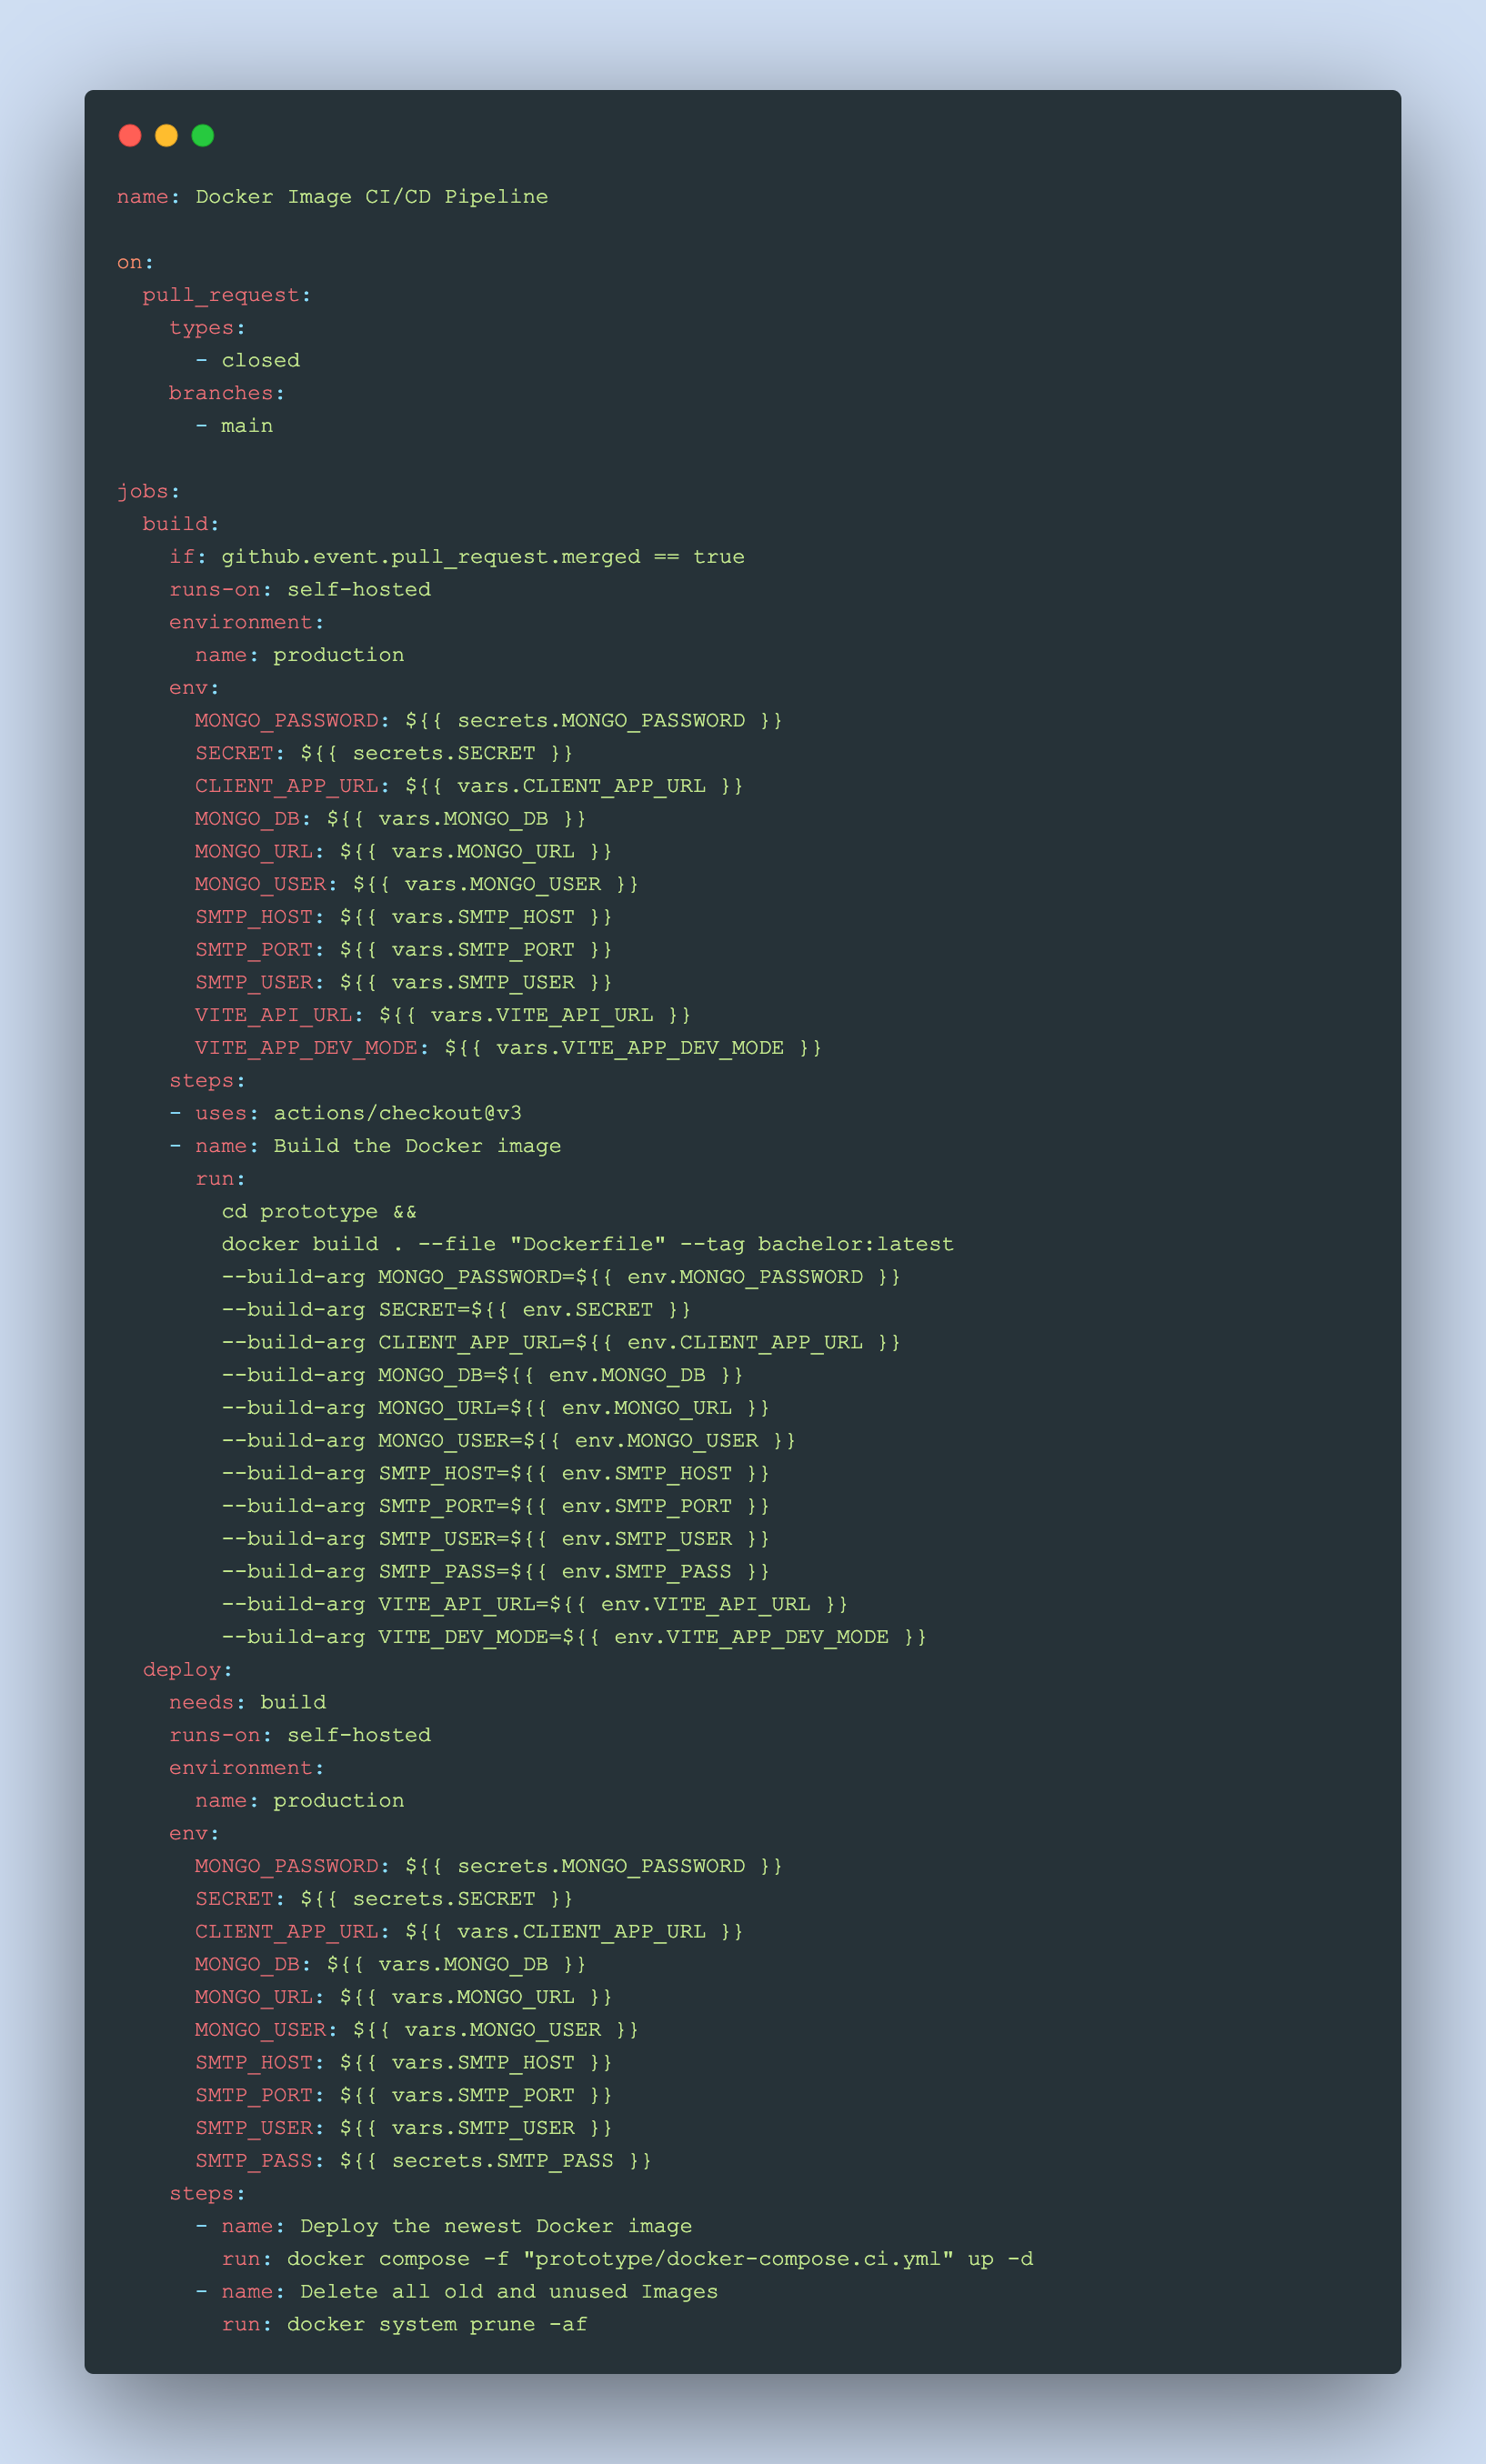
\includegraphics[width=\linewidth]{GitHubAction}
        \captionof{figure}{GitHub-Action}
    \end{minipage}
\end{center}
\vspace{20pt}

Die Pipeline besteht aus zwei Teilen, sogenannten Jobs: Build und Deploy.
Build erzeugt aus dem geupdateten Quellcode ein neues Docker-Image nach den konkreten Anweisungen die in dem Dockerfile im root-Verzeichnis des Prototypen definiert sind. Bei dem Dockerfile handlet es sich um ein multi-stage Dockerfile, welches in drei Schritten ein Image erzeugt. Diese drei Schritte sind:
frontend-build, backend-build, und production.

\vspace{20pt}
\begin{center}
    \begin{minipage}{1\linewidth}
        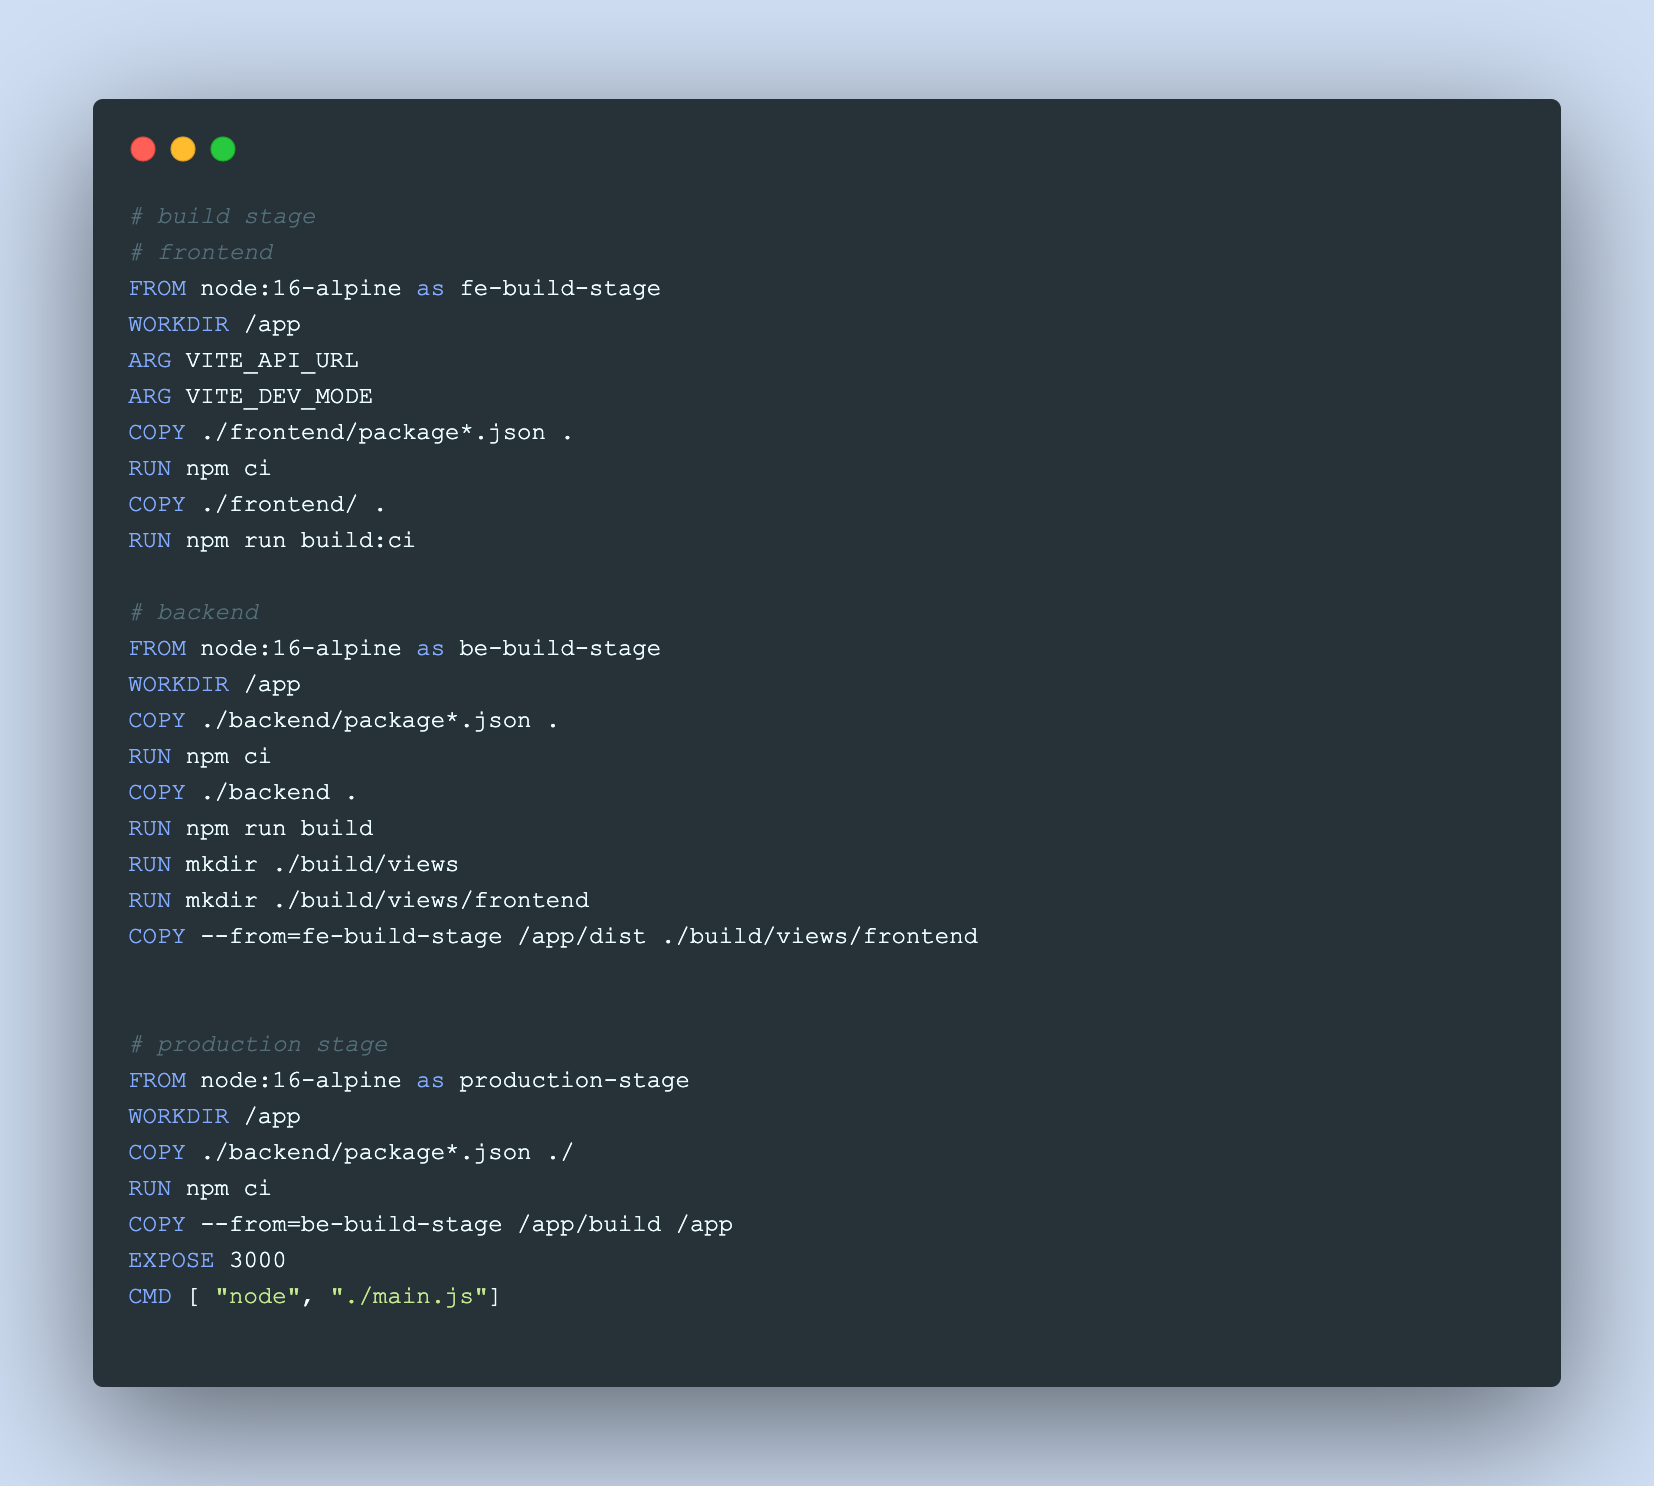
\includegraphics[width=\linewidth]{DockerFile}
        \captionof{figure}{Dockerfile zum Bauen des Images}
    \end{minipage}
\end{center}
\vspace{20pt}

Im ersten Schritt wird der Frontend-Code kompiliert. Im zweiten Schritt wird der Backend-Code kompiliert und das kompilierte Frontend aus dem ersten Schritt zur statischen auslieferung in einen bestimmten Ordner kopiert. Im dritten Schritt wird ein Node Image für die Produktivumgebung erzeugt welches das Kompilierte Backend inklusieve des Frontends enthält und mit einem Start-Befehl der Webserver gestartet wird.
Das resultierende Image, welches nun eine lauffähige Version der Anwendung enthält, wird anschließend als neueste Version des Images getagt.
Deploy führt ein Update der konkreten Produktivumgebung durch. Dazu wird das Image, welches im Build-Job erzeugt wurde, und das laufende Image ersetzt. Hierzu wird die Docker-Compose-Datei verwendet, welche die Konfiguration der Docker-Services der Produktivumgebung beschreibt. Diese Datei referenziert immer die neueste Version des gebauten Images und einen Reverse-Proxy-Service von "Traefik", welcher dazu dient das Portmapping auf dem Server zu übernehmen und ein SSL-Zertifikat für die angegebene Domain auszustellen.
Zuletzt werden alle alten und unbenutzt Images gelöscht.